\documentclass[a4paper]{article}
\usepackage{graphicx}

\usepackage{polyglossia}
\setmainlanguage{english}
\setotherlanguage{russian}
\setmainfont{FreeSerif}

\begin{document}

\title{For Whom the Bell Tolls}

\author{Sergey Feranchuk \\{\small(self-employed; residence: Smolensk, Russia; e-mail: feranchuk@gmail.com)}}

\maketitle

\begin{flushright}
{\small \textit{to my mother}}
\end{flushright}

\section{Abstract}

Речь в работе идет о соотношении периодических ритмов с нерегулярными. Более узко, для микро-экосистем почвы, периодические пожары приводят к обновлению экосистем, как и намеренное регулярное освобождение от посевов, для  сельскохозяйстенных земель. Образцы почвы, и из человека - посмотрели состав микроорганизмов. Смотрели "по крупному", обзорно.

В таком взгляде много общего, между разными сообществами микроорганизмов. То что бы можно было тут увидеть - признаки нестабильности, скрытой накопившейся нестабильности вследствии изменений режима периодичных воздействий на микро-сообщества в последние десятиления.


\par

\section{Введение}

\begin{itemize}

\item ''прорыв'' в микробиологии позволил увидеть больше в том что относися к микроорганизмам, акценты в описаниии причин и следствий привычных явлений в этом свете другие.

\item в микробных сообществах есть общее, прагматически, микроорганизмы с земли, микроорганизмы с растений и животных переносятся легко и адаптируются быстрее чем ''хозяева''.

\item что касается ''пахотного цикла'', эффект от его прекращения и сокращения, сказался бы на том общем, что есть во всех вышеупомянутых тиах сообществ.



\end{itemize}

\section{Методы}

Подробности в приложении 1.

\vskip 20pt

Таблица 1: {\textit перечислены шесть использованных образцов} 

\begin{tabular}{llll}
\hline
Порядковый номер&Описание\\
\hline
1&Англия&2003&почва\\
2&Канада&2013&почва\\
3&Израиль&2014&human/feces\\
4&Англия&2015&human/lung\\
5&Израиль&2015&soil/desert\\
6&Израиль&2019&soil/sandy\\
\hline
\end{tabular}

\section{Results}

На рисунке 1 - соотношение крупных групп организмов, состав более детально групп описан в таблице ниже.

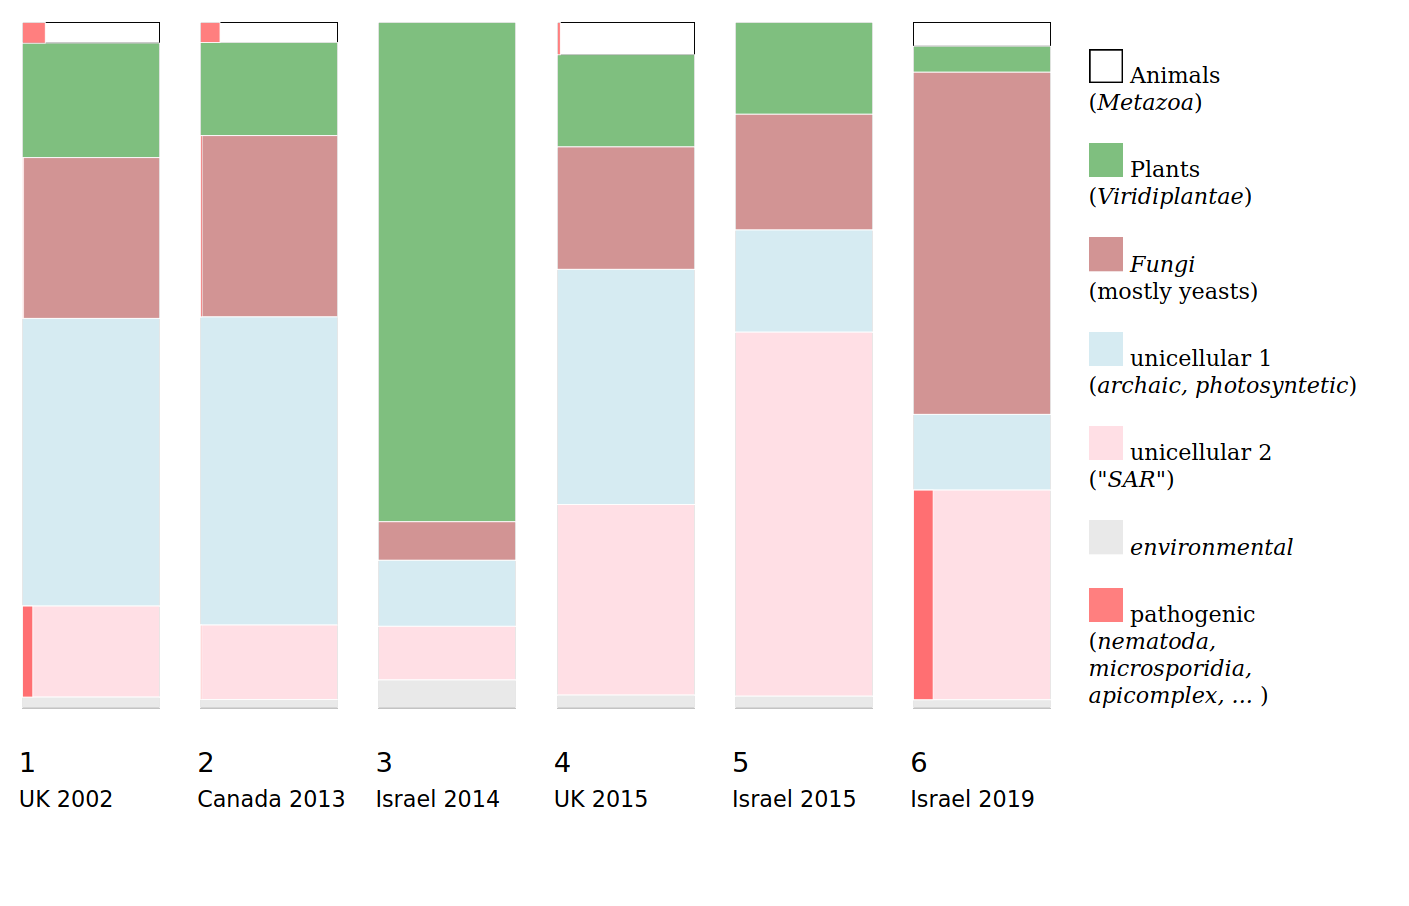
\includegraphics[width=0.9\textwidth]{tilechart.png}

Рис. 1 {\textit Соотношение состава групп организмов, по образцам - колонки соответстуют образцам}

На рисунке выделены красным и в таблице перечислены группы, включающие паразитические организмы, потенциально вызывающие хронические трудно излечимые расстройства здоровья. Их присутствие в почве невелико.

Таблица 2.

\begin{tabular}{lll}
\hline
Обозначение&Состав, как характеристика&Классы патогенов, по образцам\\
\hline
Animals&Mollusca,Arthopoda&1,6-Nematoda,4-Platyhelmintes\\
Plants&Chlorophyta,Streptophyta& \\
Fungi&95\% - 100\% Saccharomycotina (yeast)&1,2-Microsporidia\\
Unicellular 1&Euglenozoa,Rhodophyta,Haptophyta,Glaucophyta,Cryptophyta& \\
Unicellular 2&Cercozoa,Strametopiles,Alveolata&1-Apicomplexa,6-Haplosporida,Cnidaria\\
\hline
\end{tabular}

\section{Discussion}

Так называемые ''распределения численности видов'', в экологии, - по сравнению их формы можно выявить особенности экосистем, хотя из моделей для описания их формы, никакая не универсальна, как это обсуждалось в [1]. Кривые распределения численности для разных групп, по всем образцам совместно, показаны на рис. 2, и то что при этом интересует - как форма кривой соотносится с потенциальной неустойчивостью экосистемы.

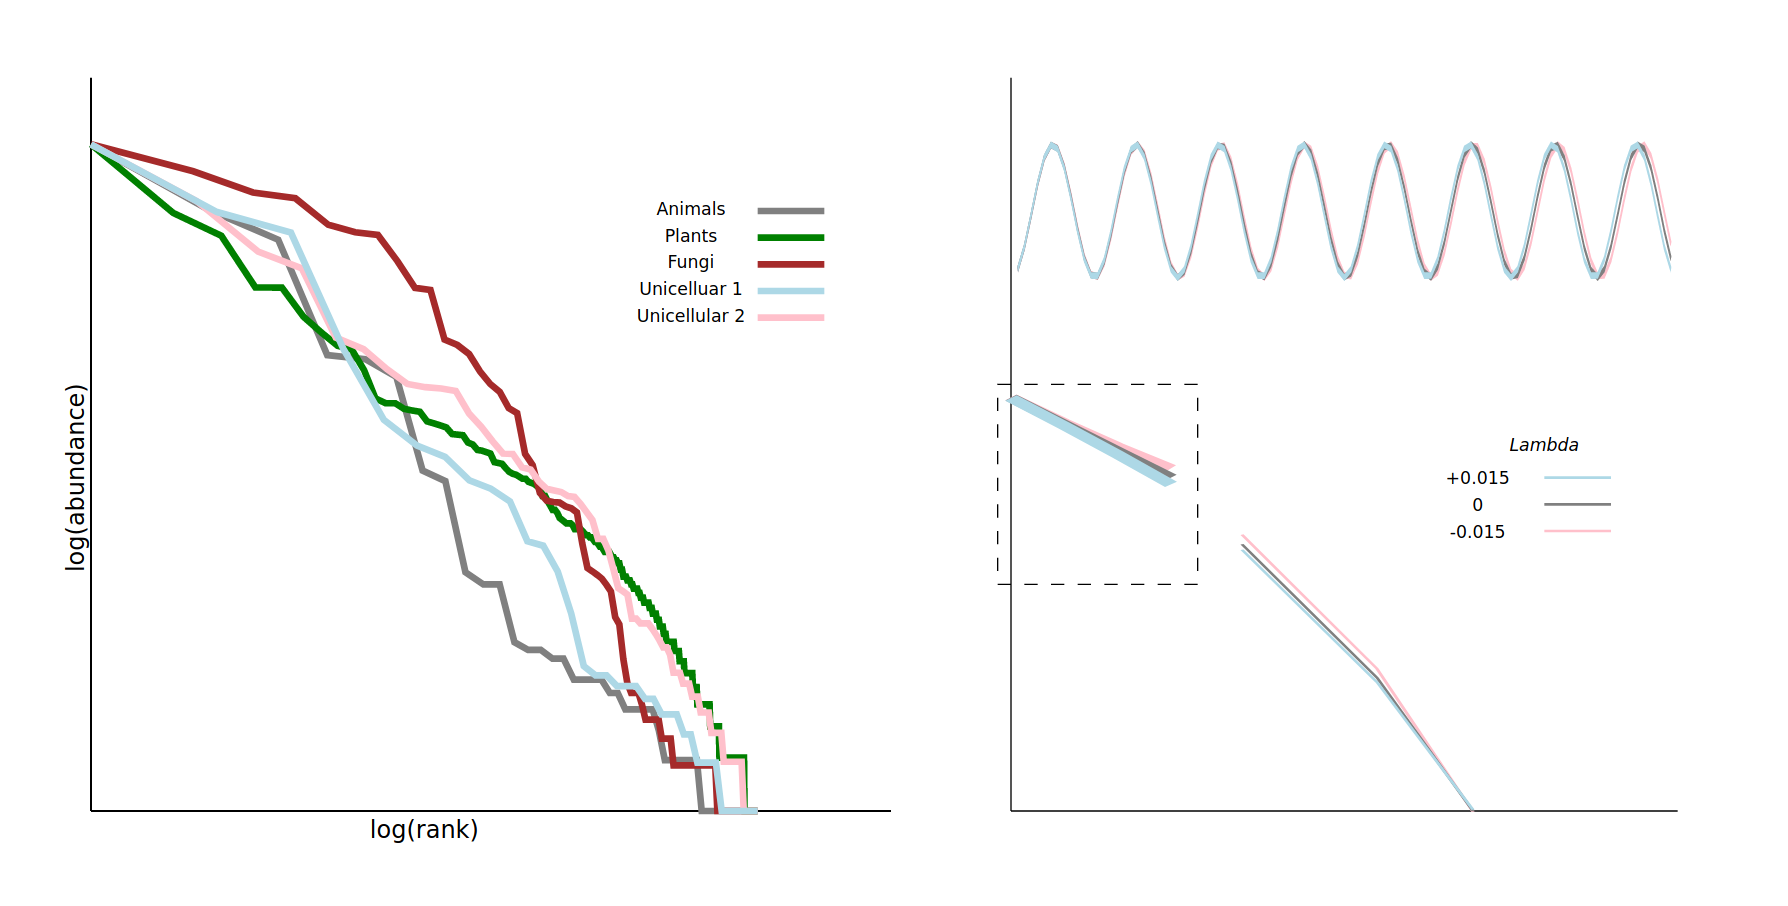
\includegraphics[width=0.9\textwidth]{rankabundance.png}


\includegraphics[width=0.3\textwidth]{rankabundance_rnaseq.png}

Рис. 2 \textit{Слева - кривые распределения численности, по группам организмов; Справа - интерпретация, смещение частоты колебаний и смещение модельных распределений численности, в модели Ципфа-Парето (обведено рамкой) и модели Больцмана, при разных знаках коэффициента $\lambda$ в ан-гармоническом осцилляторе. внизу, розовые линии - мыши на голодном пайке, по сравнению с контролем, по распределению генов  }

В форме кривых распределения численности, в болшей или меньшей степени, применимы как модель "закона Ципфа-Парето", так и модель распределения Больцмана. Обе модели, которые в других ситуациях применимы вполне явно, выражают соотношение между линейным возрастанием ''энергии'' системы, от уровня к уровню, и экспоненциальным убыванием ''заселенности'' уровней; в распределении Ципфа-Парето ''энергия'' вводится неявно и выражается по логарифмическому закону. 

Сводя вопрос сравнения численности видов к сравнению неустойчивости групп при сменах времен года, месяцев, дней и ночей, сменах дождей и яснй погоды, сменах полноводных паводков на маловодные при разливах рек - то что и определяет избыток питания в экологических нишах и под-группах, и ''заселенность'' в этих нишах - признаки искажения такой периодичности, индуцируимые через обратную связь, были бы признаком неусточивости.

Для минимально простого описания искажений периодичности, подойдет модель осциллятора с малым дополнением, внесенным в закон движения, так что в колебаниях такого ''не-гармонического'' осциллятора проявляются отклонения от гармонического закона - то что может являеться признаком потенциальной неустойчивости.

В квантовом описании, уровни энергии такого осциллятора зависят от квантового числа не вполне линейно. Используя формулу для расчета уровней энергии, предложенную в [2], через поправки к модели Ципфа-Парето и модели Больцмана на рис. 2 показано, как отклонения от периодичности проявлялись бы в кривых распределения видов.

Нарастающая периодичность соответствует положительному знаку в не-гармоничной поправке в модели осциллятора ($\hat H = p^2 + x^2 + \lambda x^4$), замедляющаяся перидичность - отрицательному знаку. Само событие кризиса в этой модели не описывается и не предсказывается. Эмпирически, колебания с нарастающим периодом - это признак риска кризиса [3]. В рамках самой модели квантового ангармонического осциллятора, ''сбой'' его движения возможен при отрицательном $\lambda$, через тоннельный переход в один из двух сегментов с отрицательной энергией за пределами области колебаний.


\section{References}

\begin{enumerate}

\item Feranchuk, S., Belkova, N., et al., Evaluating the use of diversity indices to distinguish between microbial communities with different traits. Res. Microbiol., 2018

\item Feranchuk, I., Komarov, L., et al., Operator method in the problem of quantum unharmonic oscillator, Annals of Phys., 1995 

\item Nottale, L., Scale relativity and fractal space-time: theory and applications, arxiv.org, 2008

\end{enumerate}

\section{Supplement 1}

Брали образцы где эксперимент был поставлен как полно-геномное секвенирование микробного сообщества, на секвенаторах одной и той же торговой марки. Смотрели на состав сообщества по рибосомной РНК, кроме бактерий у которых эта РНК отличается. Обработку делали в два приема - отбирали из общего пула фрагмены искомой РНК, и аккуратно сравнивали их с базой рРНК организмов, отнесенных каждый к какой-либо такономической категории согласно принятой классиификации.

Таблица S1: \textit{перечислены шесть использованных образцов} 

\begin{tabular}{lllllllll}
\hline
&Sample ID&Bases&Reads&Location&Date&type&18S RRNAs\\
\hline
1&ERR981203&5.3G&10M&51.83N 0.21E&2002.06.23&soil/meadow&1517(*)\\
2&SRR6030929&2.4G&6.1M&42.98N 81.24W&2013&soil/agricultural&125002(*)\\
3&ERR588716&8.2M&159K&Israel&2014 or earlier&human/feces&848\\
4&ERR970400&4.2G&13M&51.61N 3.95E&2015.01.01&human/lung&18747 (*)\\
5&SRR7642476&77M&128K&30.78N 34.76E&2015.08.20&soil/desert&4231\\
6&SRR12806764&48M&97K&31.86N 34.72E&2019.02.25&soil/sandy&116666\\
\hline
\end{tabular}


Таблица S2: \small{Количество аннотированных фрагментов рРНК по группам в каждом из образцов}

\begin{tabular}{lllllll}
\hline
Taxonomy(*) &1&2&3&4&5&6\\
\hline
Acanthamoebidae Acanthamoeba&2&4& &1& &\\
Alveolata Apicomplexa&12&&&14& &\\
Alveolata Ciliophora&&&&2&9&1\\
Alveolata Haplosporida&&4&&&&5406\\
Cercozoa Cercomonadida&&2&&&&\\
Cercozoa Chlorarachniophyceae&4307&197&5&108&876&14637\\
Cryptophyta Cryptomonadaceae&91&&&9&389&382\\
Cryptophyta Teleaulax&&2&&&&\\
Diplomonadida Hexamitidae&19&5&&2&&\\
environmental samples&357&50&35&25&1206&1490\\
Euglenozoa Euglenida&407&84&&46&&1\\
Euglenozoa Kinetoplastida&2072&785&4&270&1206&5343\\
Fungi Ascomycota&3343&1044&&347&11860&60992\\
Fungi Basidiomycota&&&48&3&4&\\
Fungi Chytridiomycota&&&&1&&\\
Fungi Microsporidia&1&12&&3&2&12\\
Fungi Zygomycota&5&8&&&1&\\
Glaucocystophyceae Glaucocystales&77&56&&12&2890&5020\\
Glaucocystophyceae Gloeochaetales&244&8&8&9&5042&1845\\
Granuloreticulosea Foraminifera&3&&&&&\\
Haptophyceae Isochrysidales&317&103&11&24&33&19\\
Haptophyceae unclassified Haptophyceae&17&2&&1&32&24\\
Metazoa Acanthocephala&&&&&&1\\
Metazoa Arthropoda&382&12&&13&2424&627\\
Metazoa Chordata&&2&&5&&\\
Metazoa Cnidaria&&&&&&6\\
Metazoa Mollusca&475&91&&22&8907&3641\\
Metazoa Myxozoa&&&&8&&2\\
Metazoa Nematoda&&15&&&&38\\
Metazoa Platyhelminthes&26&&&&&13\\
Metazoa Porifera&&&&&6&\\
Parabasalidea Trichomonadida&2&&&1&&\\
Rhodophyta Bangiophyceae&2962&541&43&175&714&801\\
Rhodophyta Florideophyceae&232&227&16&88&148&110\\
stramenopiles Bacillariophyta&125&47&3&10&3091&312\\
stramenopiles Chrysophyceae&41&10&1&1&3&3\\
stramenopiles Olisthodiscus&379&29&&17&28&78\\
stramenopiles Oomycetes&&2&&&&\\
stramenopiles Phaeophyceae&33&6&&&1&\\
stramenopiles Placididea&303&136&57&48&33139&17046\\
Viridiplantae Chlorophyta&1636&401&478&139&1563&2569\\
Viridiplantae Streptophyta&876&315&137&113&7886&4583\\
\hline
\end{tabular}

{\small(*) Таксономия согласно версии EBI, 2-й и 3-й уровни.}

\section{Supplement 2}

{\small команды консоли unix, использованные для обработки данных }

\subsection{18S RRNA reference base}

\small{
cat ssu\_jan03.tsv | bash -c 'while read line; do if [ ''\$\{line:0:4\}'' == "tax," ]; then if [ ''\$\{line:5:5\}'' == ''Eukar'' ]; then if [''\$f'' == ''2'' ]; then echo ''\$i" ''\$\{line:5\}; i=`echo \$i + 1 | bc`; f=''1''; fi;fi;  else if [ ''\$f'' == ''1'' ]; then if [ ''\$\{line:5\}'' != '''' ]; then echo \$\{line:5\}; f=''2''; fi; fi; fi; done; ' | awk '\{ if ( \$2 == ''Eukaryota;'' || ( p == ''Eukaryota;'' \&\& length( \$0 ) > 100 ) ) \{ print \$0 \}; p = \$2 \}' | awk '\{ if ( p != \$2 ) \{ print \$0 \}; p = \$2 \} ' >rrna\_euk.fa

cat \$sample | awk '\{ print substr( \$1, 1, length( \$1 ) - 1 ) \}' | bash -c 's='''';c=0;while read line; do if [ ''\$line'' != ''\$s'' ]; then if [ ''\$s'' != '''' ]; then echo ''\''\$s\'' : \$c,''; fi; s=\$line; c=1; else c=`echo ''\$c+1'' | bc`; fi; done;

sort \$sample |  bash -c 's='''';c=0;while read line; do if [ ''\$line'' != ''\$s'' ]; then if [ ''\$s'' != '''' ]; then echo ''\$s \$c''; fi; s=\$line; c=1; else c=`echo ''\$c+1'' | bc`; fi; done;' | awk '\{ print \$3 '' '' \$(NF-1) '' '' \$NF \}' | sort - | bash -c 's='''';b='''';c=0;while read line; do if [ ''\$\{line:0:5\}'' != ''\$\{s:0:5\}'' ]; then h=`echo \$s |awk '''''''\{print \$1\}'''''''`; echo ''\$h \$b''; c=0; s=\$\{line\}; else n=`echo \$line | awk '''''''\{print \$NF\}'''''''`; if [ \$n -gt \$c ]; then c=\$n; b=`echo \$line | awk '''''''\{ print \$(NF-1) \}'''''''`; fi; fi; done; h=`echo \$s |awk '''''''\{print \$1\}'''''''`; echo ''\$h \$b'''

}


\subsection{Processing of a sample}

\small{
head -n 4000000 \$sample.fastq >t0.fastq

sortmerna --ref ssu.fa,ssu.idx --reads t0.fastq --aligned t1 --sam

cat t1.sam | awk '{ print ''>'' \$1 ''\\n'' \$10 }' > t2.fa

blastn -db ssu.db -query t2.fa -evalue 1e-2 -task blastn -max\_target\_seqs 1 -out t3.tsv -outfmt ''6 sallseqid''
out=test-\${sample}

mv \${out}.tsv t3.tsv

cat t3.tsv | while read line; do t=`grep ''>\$line '' ssu.fa`; echo \${t:1} >>\$out.txt; done;

cat \$out.txt | awk '{ gsub(/[0-9]/,''''); gsub( ''; '', '','' ); print }' | sort >\${out}.csv

cat \$out.csv | awk -F '','' '{ print \$2 '' '' \$3 }' | bash -c 's='''';c=0;while read line; do if [ ''\$line'' != ''\$s'' ]; then if [ ''\$c'' != ''0'' ]; then echo ''  \''\$s\'' : \$c,''; fi; s=\$line; c=1; else c=`echo ''\$c+1'' | bc`; fi; done; echo ''  \''\$s\'' : \$c'';'; 

} 

\subsection{Rank-abundance} 

e.g, SAR:

grep -E 'Cercozoa|strametopiles|Alveolata|Acanthamoeba' test*.txt | sort | awk '\{ print \$1 \}' |  bash -c 's='''';c=0;while read line; do if [ ''\$line'' != ''\$s'' ]; then if [ ''\$s'' != '''' ]; then echo \$c; fi; s=\$line; c=1; else c=`echo ''\$c+1'' | bc`; fi; done; echo \$c' | sort -g | awk '\{ s = \$0 '' '' s \} END \{ print s \}' | awk '\{ s = ''''; for ( i=1; i <= NF; i++ ) \{ s = s '' '' log(i)/log(NF) '','' log(\$i)/log(\$1) \}; print s \}'

\subsection{Unharmonic oscillator}

classical system:
{\texttt \small
awk '\{ lambda=\$1; x = 1; v = 0; dt = 0.01; s = ''''; for ( i = 1; i < 5000; i++ ) \{ x = x + v * dt; v = v - x * ( 1 + lambda * x * x ) * dt; if ( i \% 50 == 0 ) \{ s = s '' '' ( i * dt ) '','' x; \}; \}; print s \}' 
}

C code:

{\texttt \small
void solve\_cubic( double h, double g, double *e1 ) \{ double d = atan2( sqrt( pow( h, 3 ) - g * g ), -g ) / 3.;   double c = sqrt( h ) * cos( c );  *e1 = 2 * c; \}

    
int main( int argc, char **argv ) 
\{  
    double lambda = atof( argv[1] );
    double nmax = atoi( argv[2] );
    double omega\_n;    
    int n;
    for ( n = 0; n < nmax; n++ )
    \{
        solve\_cubic( 1. / 3., -3. * lambda * ( 1. + 2. * n + 2. * n * n ) / ( 1. + 2. * n ), \&omega\_n );
        printf( ''\%.2f '', ( 1. / 4. ) * ( 3. * omega\_n + 1. / omega\_n )* ( n + 1. / 2 ) );

    \}
 \}
}
 
\subsection{Rna-seq}

fractal dimension:

{\texttt \small
awkcmd='\{ n1 = abs( \$1 - \$2 ) + abs( \$2 - \$3 ) + abs ( \$3 - \$4 ) + abs(  \$4 - \$5 ) + abs( \$5 - \$6 ); n2 = 0.5 * ( abs(  \$1 - \$3 ) + abs( \$2 - \$4 ) +  abs(  \$3 - \$5 ) + abs( \$4 - \$6 ) ); n3 = 0.3333 * ( abs(  \$1 - \$4 ) + abs( \$2 - \$5 ) + abs( \$3 - \$6 ) ); l2 = log(2 ); l3 = log( 3 );  if ( n1 > 0 \&\& n2 > 0 \&\& n3 > 0 ) \{ y = log( n1 ) + log( n2 ) + log( n3 ); b = ( 3 * ( log( n3 ) * l3 + log( n2 ) * l2 ) - y * 1.79 ) / 1.84; a = ( y - b * 1.79 ) / 3; d1 = log( n1 ) - a; d2 = log( n2 ) - a -b * l2; d3 = log( n3 ) - a - b * l3; sumd = d1 * d1 + d2 * d2 + d3 * d3; if ( sumd < 0.01 ) \{ print abs(b) \} \}  \} function abs( v ) \{ if ( v > 0 ) \{ return v; \} else \{ return -v; \} \}'

fdim=`awk ''\$awkcmd'' | sort -g | head -n \$median | tail -n 1`
}

\end{document}
